\documentclass[a4paper,12pt]{article}

% 导言区
\usepackage{titlesec}
\usepackage{lipsum} % 示例用,可以删除
\usepackage{geometry}
\usepackage{setspace}
\usepackage{amsmath} % 用于数学公式
\usepackage{graphicx} % 用于插入图片
\usepackage{float}
\usepackage{lipsum} % 用于生成虚拟文本
\usepackage{ctex} % 导入 ctex 包以支持中文
\usepackage{titlesec} % 导入 titlesec 包以定制标题样式
\usepackage{fontspec} % 用于设置中文字体
\usepackage{amsfonts}
\usepackage{amsmath} % 提供 \text 和 \tanh 命令
\usepackage{bm}      % 提供 \bm 命令用于粗体
% 目录设置
\usepackage[nottoc,notlot,notlof]{tocbibind}
\usepackage{enumitem}
% 页面设置
\geometry{margin=1in}

% 标题设置
\titleformat{\section}{\normalfont\Large\bfseries}{\thesection}{1em}{}
\titleformat{\subsection}{\normalfont\large\bfseries}{\thesubsection}{1em}{}
\titleformat{\subsubsection}{\normalfont\normalsize\bfseries}{\thesubsubsection}{1em}{}

% 行间距设置
\onehalfspacing

% 文档信息
\title{商业模式评估}
\author{需求不寄小分队}
\date{\today}

\begin{document}

    \maketitle

% 添加目录
    \tableofcontents


    \subsection{团队成员}
    211250124 程智镝

    211250122 刘辉

    211250159 陈凌

    211250158 李忠信
    \subsection{度量数值}

    \section{文档简介}
    

    \section{商业模式环境}
    
    
    \section{商业模式总体评估}
    

    \section{SWOT分析}
    \subsection{S\&W}
    \subsubsection{打分结果:}
    \begin{figure}[htbp]
        \centering
        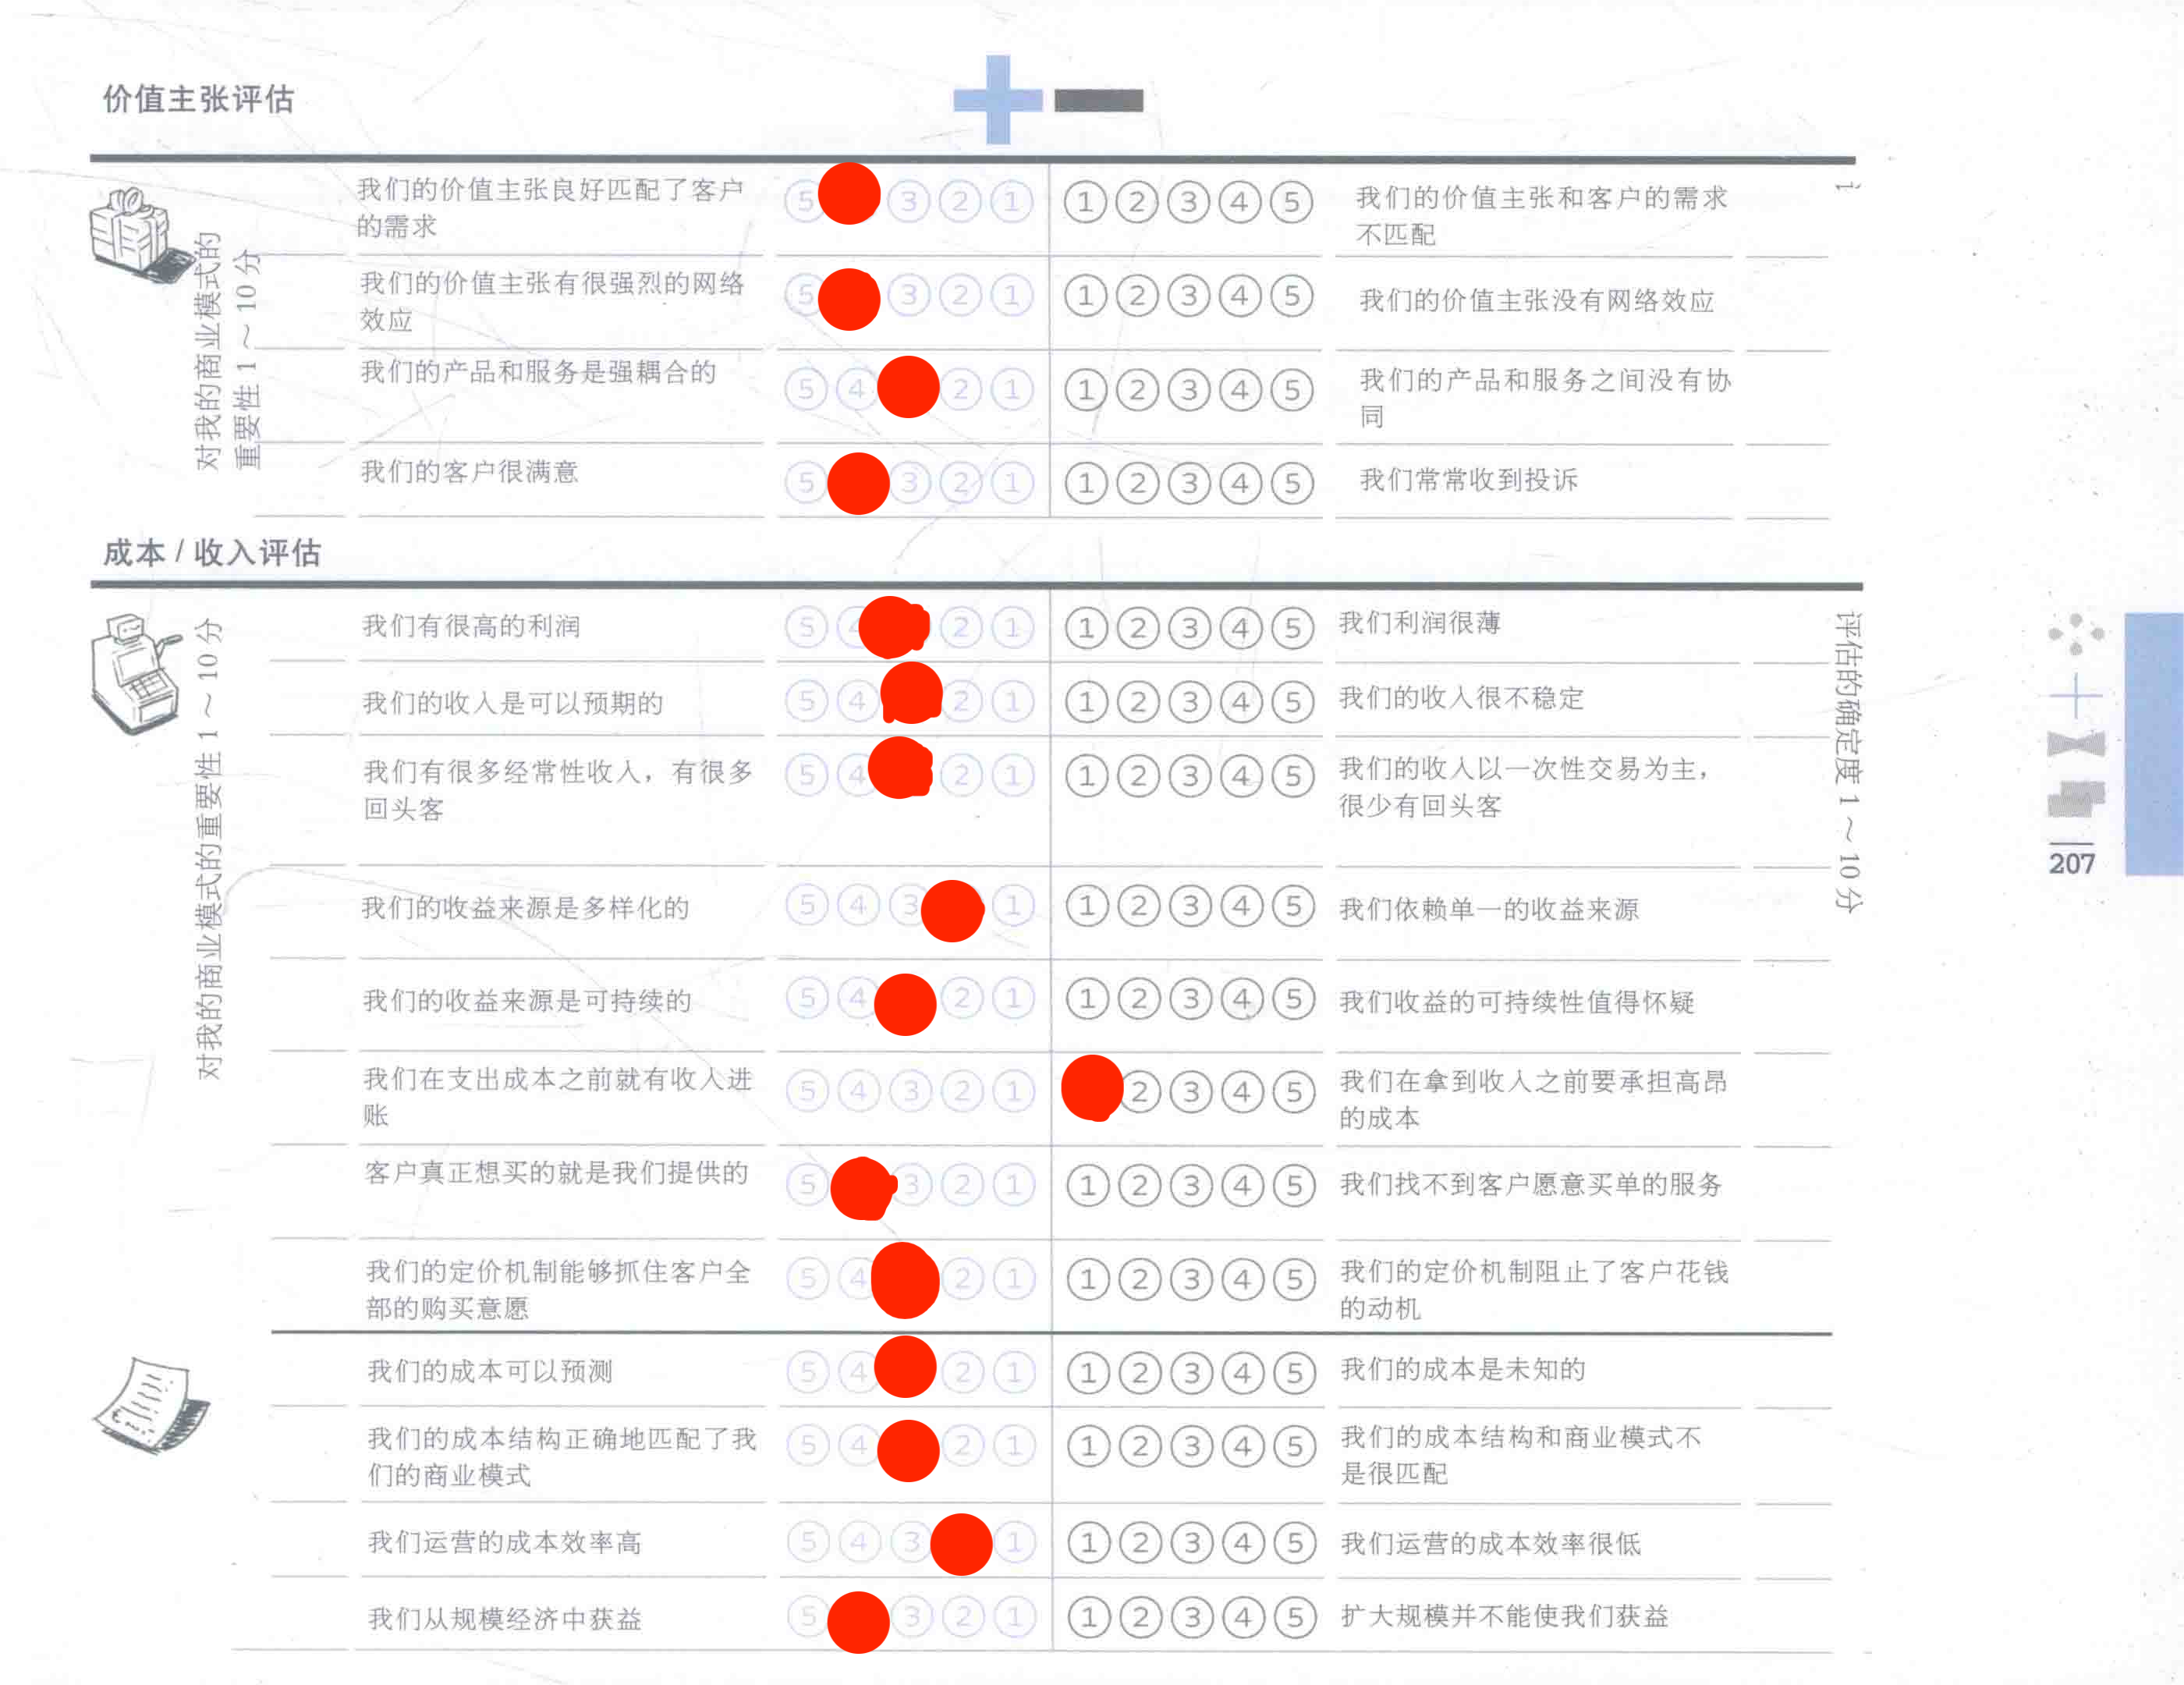
\includegraphics[width=15cm,height=25cm]{S&W1.png}
    \end{figure}
    \begin{figure}[htbp]
        \centering
        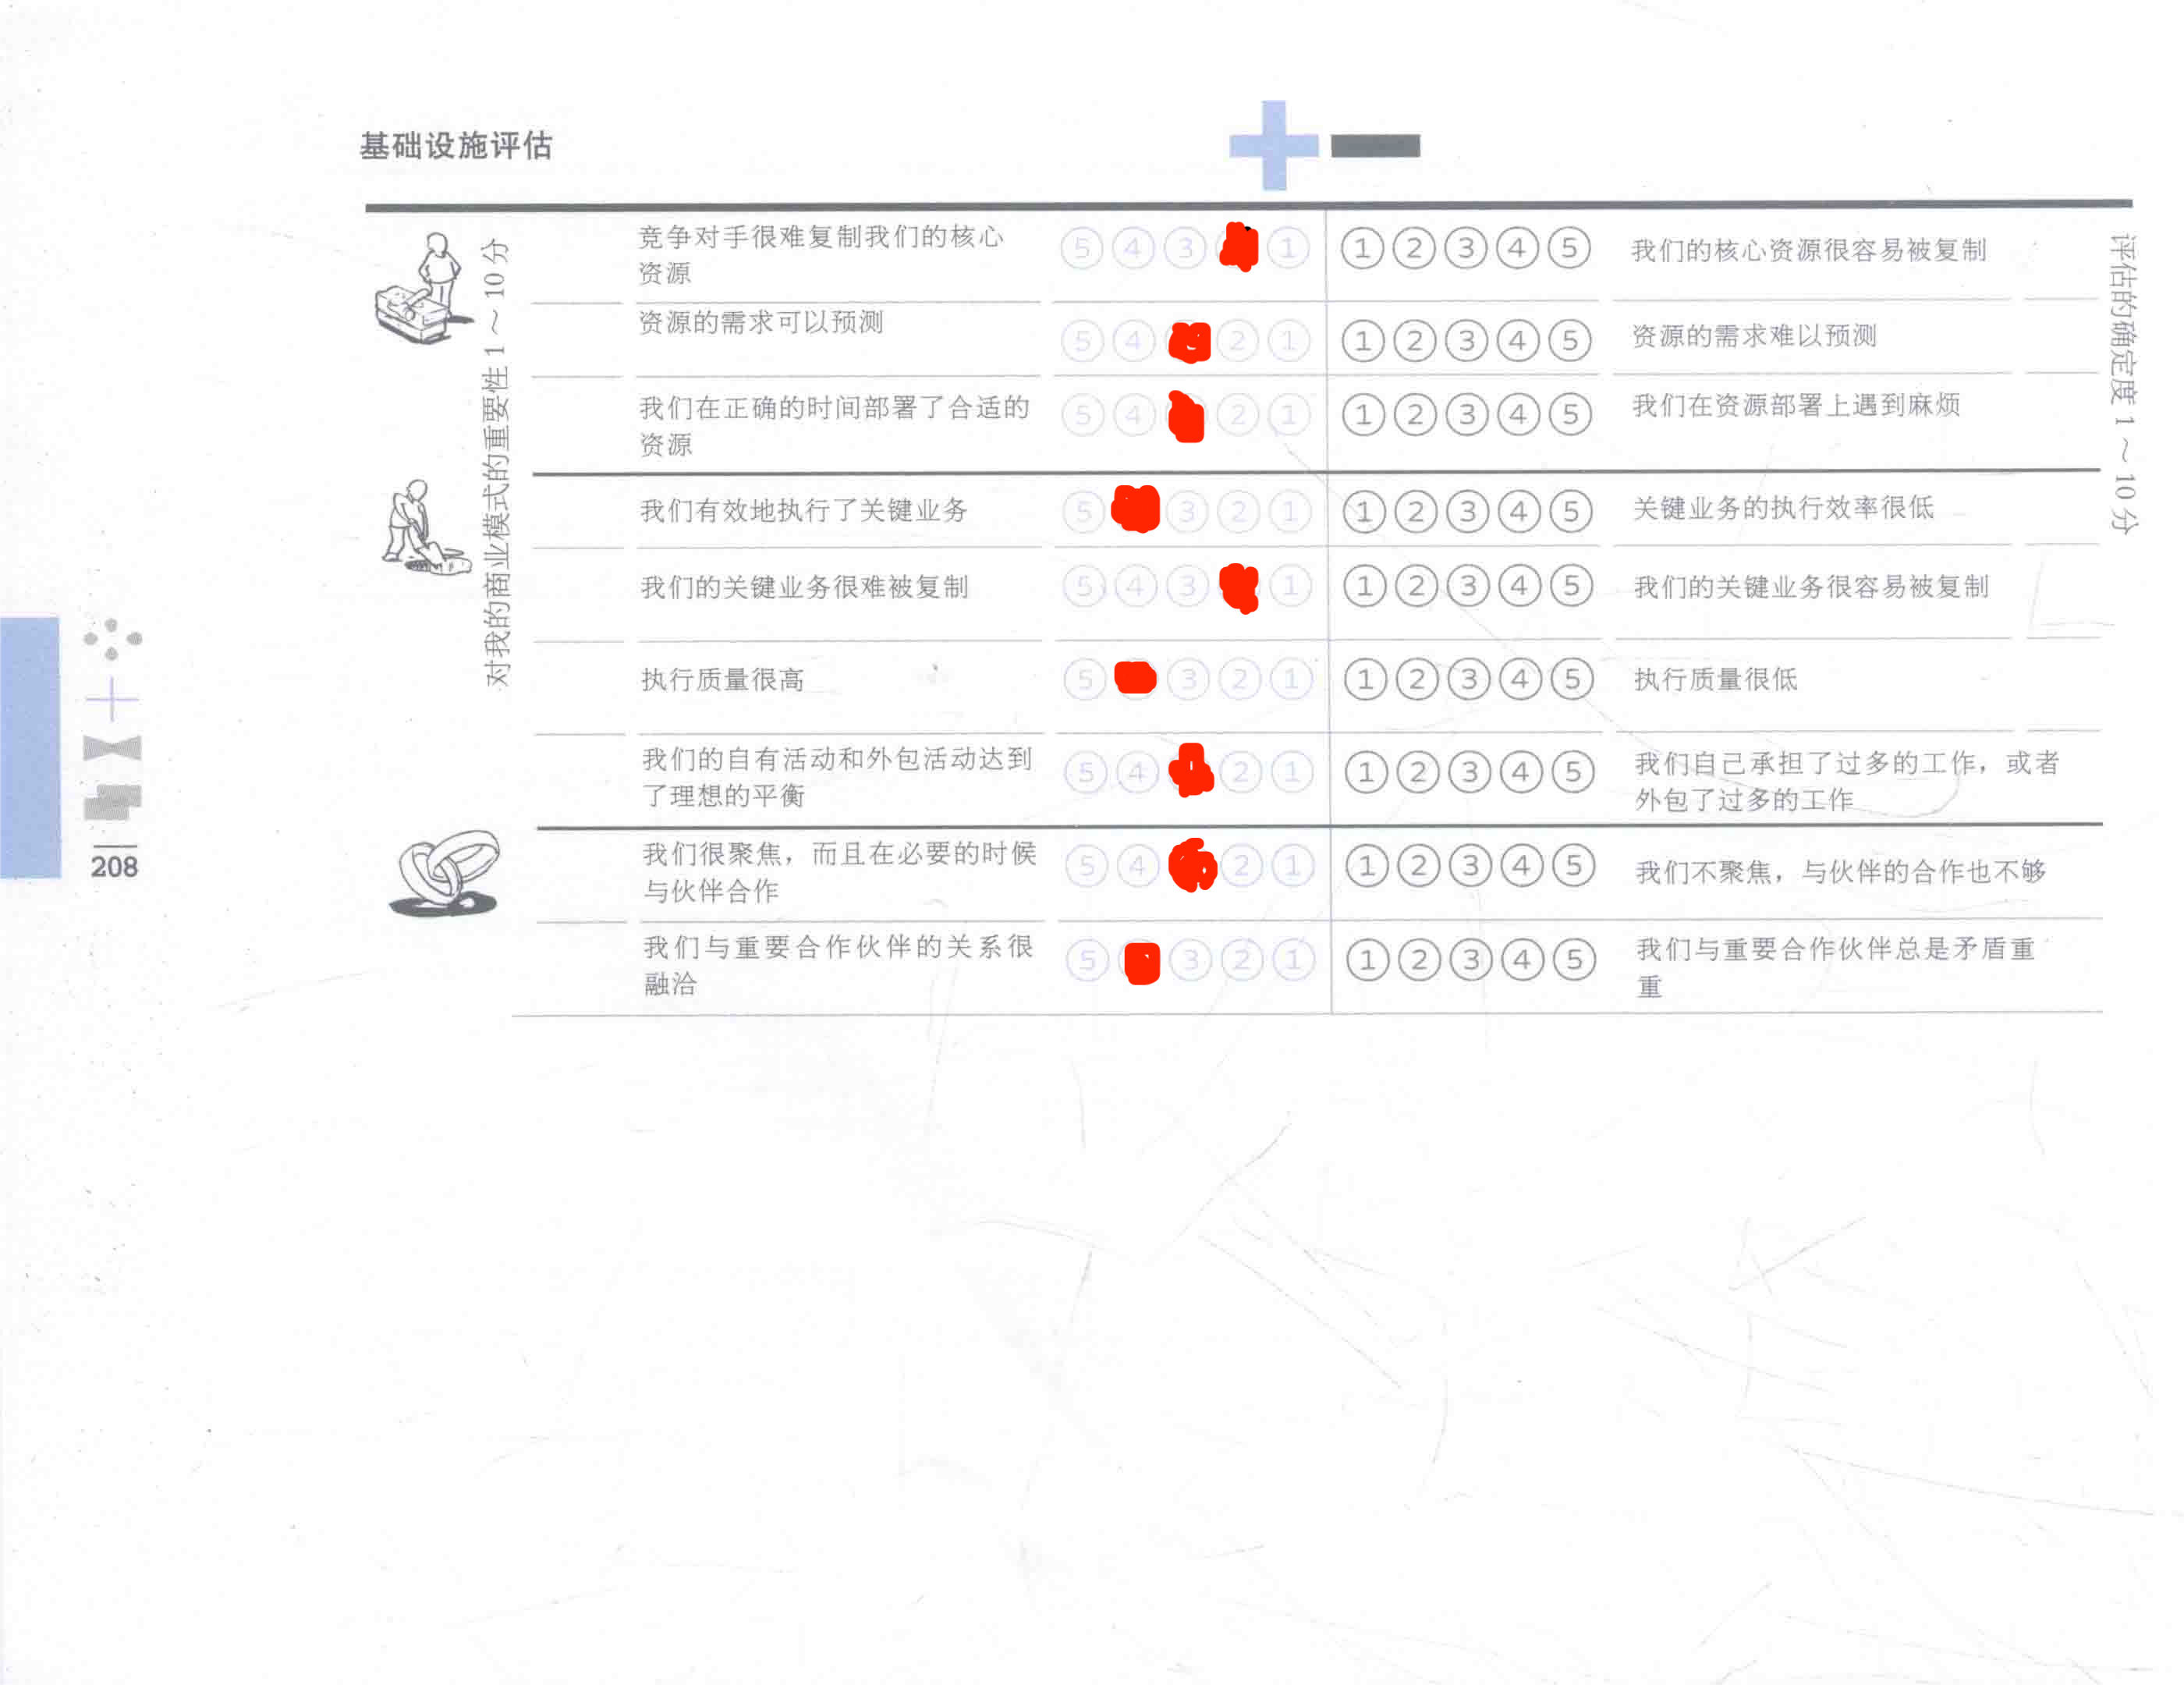
\includegraphics[width=15cm,height=25cm]{S&W2.png}
    \end{figure}
   
    \begin{figure}[htbp]
        \centering
        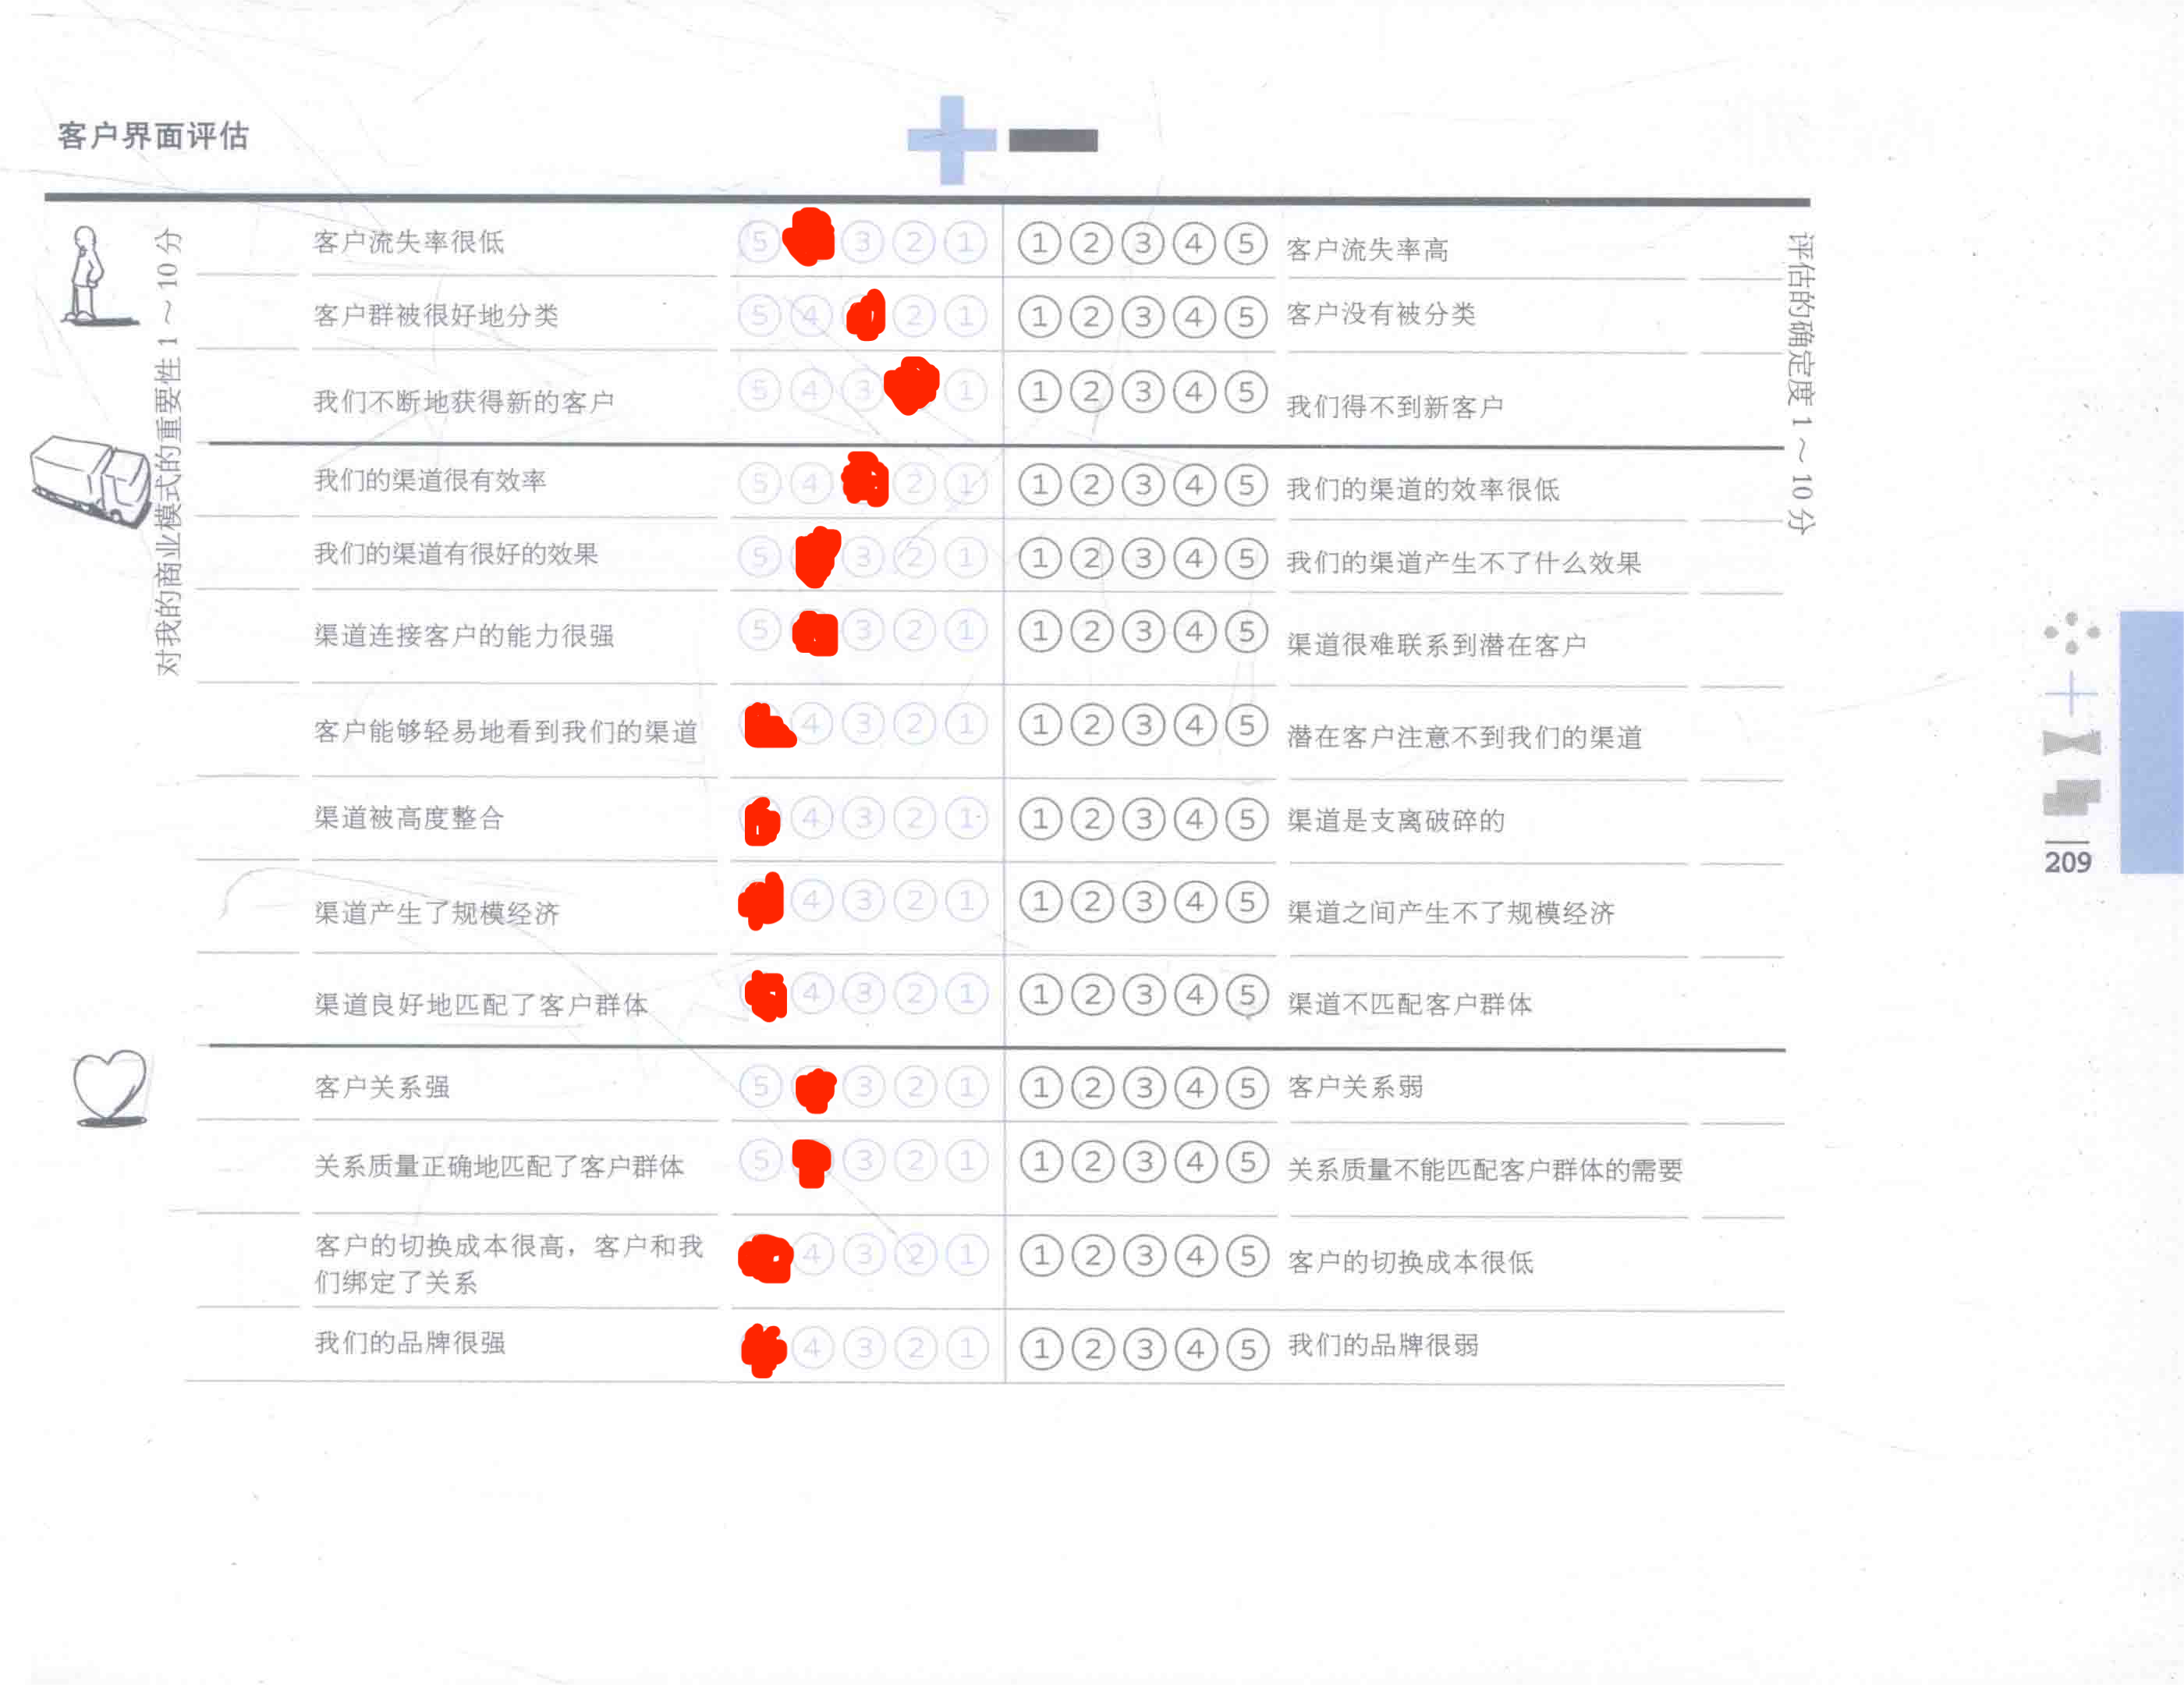
\includegraphics[width=15cm,height=25cm]{S&W3.png}
    \end{figure}
    \clearpage % 强制图片开始新页面
    \subsubsection{价值主张评估}
    \texttt{腾讯会议的独特价值主张}

\begin{itemize}
  \item 腾讯会议产品的价值主张旨在与客户需求紧密契合。他们始终站在客户的角度,深入了解他们真正需要的服务。
  
  \item 提供免费的会议服务,确保普通用户能够轻松享受舒适的会议体验。
  
  \item 为需要更个性化设置、更长时间、更多参会人数以及更大云存储空间等功能的用户提供收费的VIP服务。
  
  \item 面向企业用户提供高级企业会议服务;同时,为学者用户提供专属的“自习室”和网络研讨会议。
  
  \item 始终坚持“对症下药”的原则,以用户为中心,通过收集用户反馈不断优化腾讯会议产品,以满足他们的合理需求。
\end{itemize}

\texttt{腾讯会议的强大网络效应}

\begin{itemize}
  \item 腾讯会议的价值主张具有显著的网络效应。产品的价值取决于使用该产品的其他用户数量,即网络外部性或网络效应。
  
  \item 腾讯会议虚拟会议软件是一个典型的具有网络效应的产品。在刚开始运营时,他们面临高昂的运营成本,并且用户只能与数量有限的人交流信息和使用经验。
  
  \item 随着口碑的积累和知名度的提高,他们将有足够的流水来支付成本并逐渐实现盈利。同时,随着客户数量的增多,像公开会议这种需要大量潜在用户群体的服务也能有效提高腾讯会议产品本身的价值。
  
  \item 因此,腾讯会议的价值主张具有强烈的网络效应。
\end{itemize}

\texttt{腾讯会议的高度耦合产品和服务}

\begin{itemize}
  \item 腾讯会议虚拟会议软件的存在旨在为用户提供仿真实的会议服务。他们追求通过产品为顾客提供最真实、最自然、最愉悦的服务,因此,可以说他们的产品和服务之间存在密切的关系。
\end{itemize}

\texttt{腾讯会议的客户满意度保障}

\begin{itemize}
  \item 他们确信腾讯会议的客户将会非常满意。腾讯会议虚拟会议软件不断追求卓越的用户体验。一旦用户提出不满意的反馈,他们会进行权衡和测试,在经过权衡和测试之后,会做出相应的优化⽅案。
\end{itemize}
\textbf{调研:}
\begin{itemize}
    \item 腾讯会议准备从‘产品的专业能力与体验’进化到‘建设开放生态’,将以更专业、开放的姿态,引入更多的伙伴,更好的服务行业与客户。--《如何理解腾讯会议3.0“会聚力”的价值主张》
    \item 腾讯会议企业版将推出混合云部署,混合云部署更加灵活、稳定,能够方便企业管理员的远程运维,更提高了大型企业的使用感受,内部会议可以部署在专有云上,保证信息资产安全。--《服务3亿用户、14亿场会,腾讯会议企业版迎来重大升级》
    \item 腾讯会议作为在线办公软件中的一匹黑马,自2019年底发布以来就出现了高速增长,仅仅上线两个月内,每日活跃用户就超过1000万,一举成为中国最多视频会议产品,助力全球抗击疫情。--《有人给腾讯会议算了一笔账,5个月节约社会成本高达714亿元》
\end{itemize}
\subsubsection{成本收入评估}
\texttt{腾讯会议较高的利润。}
腾讯会议旗下有众多vip才能享受的服务,这些服务有很多是中大型企业经常甚至必须使用到的,腾讯会议在重视用户体验和口碑的同时,
也会收取相应的费用,对于不经常使用的用户完全可以只使用免费服务即可,腾讯会议的收费功能更多的是面向那些经常要开展大型会议的中大型企业,或者对
线上学术研讨有强烈需求的教育机构等。他们一次会议的人数众多,时间较长,对腾讯会议vip提供的服务有较强的依赖性。他们的vip服务主要分为三个档次:个人会员版、商业版、企业版。针对不同客户都有让他们难以割舍的服务。\\

\texttt{腾讯会议的收入基本是可以预期的。}在VIP会员费板块,通过引⼊年卡、连续包⽉等⽅式
保证收⼊的可预期性。同时和教育机构以及⾼校、企业的合作往往都是⻓期的,从中收取
的相应的团体专属使⽤权的购买费⽤⾃然是可以预期的。当然,也存在像云存储使⽤费这
样的可预期性⼀般的收⼊,也尽可能的会去通过⼀次性购买⾜量的云存储空间给予折
扣的⽅式来提⾼其可预期性。\\

\texttt{腾讯会议有很多经常性的收入,有很多回头客的。}腾讯会议提供的VIP服务是具备⽤户黏性的,他们以⽤户为中⼼的主旨会使他们在留住⽤户这⼀块有着较强的⾃信,再加上引⼊的连续包
⽉的机制,可以保证收⼊的经常性。任何回头客都是建⽴在产品对⾃⼰有⾜够的吸引⼒之
上的,不断优化的舒适的使⽤体验是他们最⼤的竞争⼒,也是他们留住⽤户、并从⽤户群
体中获得经常性收⼊的保证。其中的会议字幕翻译、实时转译功能对某些跨国企业有非常大的吸引。
\\
\texttt{腾讯会议收⼊来源是多样的。}基本的收益包括:从个⼈VIP⽤户⼿中收取的VIP服务费,向教育机构、⾼校与企业收取相应的团体专属使⽤权的购
买费⽤,对有拥有更⼤的云存储空间的需求的⽤户提供云空间按存储字节的收费,还包括临时增加会议时长的费用。
\\
\texttt{腾讯会议的收入是可持续的。}正如前⾯所说,腾讯会议提供的VIP服务是具备⽤户黏性的,合理的价格
并且绝对舒适的使⽤体验,有大量实用的服务功能,可以让⽤户难以脱离使⽤VIP服务。
\\
\texttt{腾讯会议拿到收⼊之前实际上要承担较为⾼昂的成本。}产品软件的制作本身是需要投⼊⼤量的成本的,再加上腾讯会议对⽤户舒
适实⽤体验的追求,势必会有更⼤的研发⽀出。再加上在产品投⼊市场的初期,是需要通
过⼤量⼴告宣传的⽅式来增加知名度、吸引⽤户的,他们所要⽀付的⼴告费也是价格不菲
的。而且维护用户数据的大型数据库的租用或者购买、分布式系统的部署、运行服务的服务器,这些都是非常大的成本。
因此在拿到收⼊之前实际上整体是要承担较为⾼昂的成本的。
\\
\texttt{客户真正想买的就是腾讯会议提供的产品和服务。}腾讯会议是以⽤户为中⼼的,他们重视⽤户的使
⽤体验和⼝碑的积累,即使是对普通的⽤户也会给予他们⾜够舒适的使⽤体验,这些是为普通用户提供的。个性化设置、更⻓会议时间、更多⼤参会⼈数、
更⼤的云存储空间等,他们提供VIP服务的购买,这些功能对某些对远程会议有粘性需求的企业、个人都是非常有吸引力的,而且还会根据用户的反馈来进行优化整改。
\\
\texttt{腾讯会议的定价机制基本能够抓住客户的购买意愿。}腾讯会议大致上分了三类vip用户:个人会员版、商业版、企业版。个人版30元/月具有更丰富的虚拟背景、会聚模式场景、自动会议纪要、实时转写等功能。单场会议最高可容纳100/300/500人,可同时开启视频人数为60/300/500人,可根据规模做选购。
商业版4788元/年起,中小企业可以选购腾讯会议商业版,商业版提供最高2000人会议室、200G的云录制空间、直播功能、可视化数据分析、会管会控能力等功能,满足企业日常管理的需求。
企业版有较大的灵活性,企业版有更强大的协作、会管会控及企业会议管理能力,最高2000人会议室、无限云录制空间、企业仪表盘等功能,并基于API无缝与企业业务系统融合。具体价格根据企业选定服务。
\\
\texttt{腾讯会议的成本在⼀定程度上是可以预测的。}
腾讯会议的成本包括带宽和服务器成本、运营成本以及附加功能收费等。

腾讯会议需要承担高昂的带宽和服务器成本。视频会议需要大量的数据传输和存储,因此需要高速的网络和强大的服务器来支持。这些成本对于腾讯会议来说是非常高昂的,尤其在用户数量激增的情况下,服务器和带宽的需求也会相应增加。

腾讯会议还需要承担运营成本。除了服务器和带宽成本之外,腾讯会议还需要支付员工工资、市场营销、技术支持等方面的费用。这些成本也是非常高昂的,尤其在竞争激烈的市场环境中,腾讯会议需要不断投入资金来保持领先地位。

腾讯会议通过收取附加功能费用来弥补成本。腾讯会议提供了一些高级功能,例如云录制、同声传译等,这些功能需要额外的开发和技术支持成本。腾讯会议通过向用户收取这些功能的费用来弥补成本。
\\
\texttt{腾讯会议成本结构基本可以匹配他们的商业模式。}
1. 免费使用:腾讯会议的基础功能免费提供给用户,这有助于吸引大量用户,从而形成网络效应。
2. 付费增值服务:腾讯会议提供付费的增值服务,如更高质量的视频和音频、更长的会议时间、更多的会议参与者等。这些服务可以满足不同用户的需求,提高用户体验。
3. 跨平台支持:腾讯会议支持多种设备,如PC、手机、平板等,方便用户随时随地参加会议。

这些特点使得腾讯会议的成本结构可以匹配多种商业模式,具体来说:

1. 免费+广告模式:腾讯会议可以通过在免费版本中投放广告来获得收入。这种模式适用于那些希望通过广告宣传自己的品牌和产品的公司。
2. 付费订阅模式:腾讯会议可以通过提供付费的增值服务来获得收入。这种模式适用于那些需要更高质量服务的用户,如企业用户。
3. 合作伙伴模式:腾讯会议可以与其他企业合作,提供定制化的远程会议解决方案。这种模式适用于那些需要特殊功能的用户,如政府部门、金融机构等。
\\
\texttt{腾讯会议运营的成本效率相对较低。}腾讯会议一年的运营成本至少大几十个亿。 而腾讯会议几年来的营收非常有限,仅有数亿元规模。 这对于大几十亿的成本,可以说杯水车薪。\\
\texttt{腾讯会议是要从规模经济中获益的。}规模经济是企业产品绝对量增加时,其单位成本下降。
通俗的来说就是扩⼤经营规模可以降低平均成本,从⽽提⾼利润⽔平。这其实就是他们的主
要盈利模式,他们开发最初版本的成本是他们成本的⼤头,他们只有在拥有了⾜够的⽤
户,并从他们身上获利之后,才能降低他们的单位成本,也就是“摊薄”成本,从⽽他们的
利润也会在⽤户规模不断扩张的过程中不断的增⻓、提⾼。
\textbf{调研:}
\begin{itemize}
    \item 腾讯会议是一款月活跃用户过亿的在线办公软件,他拥有庞大的年轻的、高质量用户群体,他积极运用其广告能力,能够帮助广大品牌深度触达办公场景人群,凭借更沉浸式的互动广告玩法,有效解决“吸引消费者注意力”难题。--《腾讯会议如何盈利?》
    \item 受疫情影响,企业数字化转型迫在眉睫,使得轻量化SaaS服务快速普及:腾讯会议、腾讯企点和企业微信等应用都在去年实现了较高速度增长。--《腾讯2020年财报:腾讯会议跻身中国No.1,加速提升市场渗透率》
    \item 腾讯会议开放了覆盖会议邀约、会中管理、会后沉淀等相关功能超 300 个 API 接口,数千家企业组织基于腾讯会议开放提供的 API 接口,进行商业会议讨论,日均调用次数过千万。此外,腾讯会议合作伙伴已超过了 300 家,比去年增加了 2 倍有余,今年上半年腾讯会议代理收入同比增长近 200\%。--《用户突破 4 亿!腾讯会议接入混元大模型》
\end{itemize}



\section{蓝海战略}
    

\section{更新过的商业模式画布}


    
\end{document}
